\documentclass[tikz]{standalone}
% Waypoints the edge editor writes (M2b, D47). Each "coordinate" records
% where a point of a path lands, so the interpreter can be checked against
% pdfTeX: relative points after a bare node start from its centre; "+" keeps
% the base and "++" moves it; perpendicular points; pos on |- and -|
% (0.5 is the corner); a coordinate with no operation before it moves;
% and a path's own scale applies to relative points, dimensioned or not.
\tikzset{every node/.style={draw, minimum width=1cm, minimum height=6mm}}
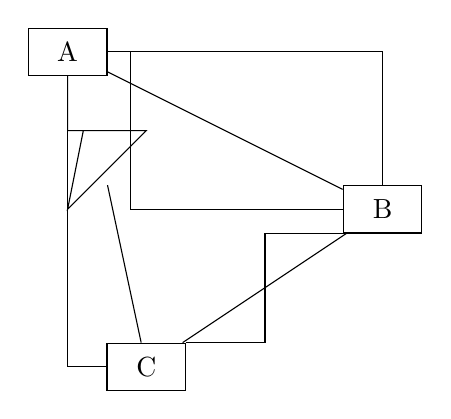
\begin{tikzpicture}
  \node (a) at (0,0) {A};
  \node (b) at (4,-2) {B};
  \node (c) at (1,-4) {C};
  \draw (a) -- ++(8mm,0) coordinate (w1) |- (b) coordinate[pos=0.5] (w2);
  \draw (a) -- ++(0,-1) coordinate (w3) -- +(1,0) coordinate (w4) -- +(0,-1) coordinate (w5) -- ++(2mm,0) coordinate (w6);
  \draw (a.east |- b.north) coordinate (w7) -- (c);
  \draw (a) -| coordinate[pos=0.25] (w8) (b);
  \draw (a) |- coordinate[pos=0.75] (w9) (c);
  \draw (a) -- (b) (c) -- coordinate[midway] (w10) (b);
  \draw[scale=2] (a) -- ++(5mm,0) coordinate (w11) -- ++(0.5,0) coordinate (w12);
  \draw (c.north east) -- ++(1cm,0) coordinate (w13) |- (b.south);
\end{tikzpicture}
